\FChapter{Chapter Twenty-Eight}{28}

\Lettrine{T}{wo} \textsc{days are passed.} It is a summer evening; the coachman has set me
down at a place called Whitcross; he could take me no farther for the
sum I had given, and I was not possessed of another shilling in the
world. The coach is a mile off by this time; I am alone. At this
moment I discover that I forgot to take my parcel out of the pocket of
the coach, where I had placed it for safety; there it remains, there it
must remain; and now, I am absolutely destitute.

Whitcross is no town, nor even a hamlet; it is but a stone pillar set up
where four roads meet: whitewashed, I suppose, to be more obvious at a
distance and in darkness. Four arms spring from its summit: the nearest
town to which these point is, according to the inscription, distant ten
miles; the farthest, above twenty. From the well-known names of these
towns I learn in what county I have lighted; a north-midland shire, dusk
with moorland, ridged with mountain: this I see. There are great moors
behind and on each hand of me; there are waves of mountains far beyond
that deep valley at my feet. The population here must be thin, and I
see no passengers on these roads: they stretch out east, west, north,
and south---white, broad, lonely; they are all cut in the moor, and the
heather grows deep and wild to their very verge. Yet a chance traveller
might pass by; and I wish no eye to see me now: strangers would wonder
what I am doing, lingering here at the sign-post, evidently objectless
and lost. I might be questioned: I could give no answer but what would
sound incredible and excite suspicion. Not a tie holds me to human
society at this moment---not a charm or hope calls me where my
fellow-creatures are---none that saw me would have a kind thought or a
good wish for me. I have no relative but the universal mother, Nature:
I will seek her breast and ask repose.

I struck straight into the heath; I held on to a hollow I saw deeply
furrowing the brown moorside; I waded knee-deep in its dark growth; I
turned with its turnings, and finding a moss-blackened granite crag in a
hidden angle, I sat down under it. High banks of moor were about me;
the crag protected my head: the sky was over that.

Some time passed before I felt tranquil even here: I had a vague dread
that wild cattle might be near, or that some sportsman or poacher might
discover me. If a gust of wind swept the waste, I looked up, fearing it
was the rush of a bull; if a plover whistled, I imagined it a man.
Finding my apprehensions unfounded, however, and calmed by the deep
silence that reigned as evening declined at nightfall, I took
confidence. As yet I had not thought; I had only listened, watched,
dreaded; now I regained the faculty of reflection.

What was I to do? Where to go? Oh, intolerable questions, when I could
do nothing and go nowhere!---when a long way must yet be measured by my
weary, trembling limbs before I could reach human habitation---when cold
charity must be entreated before I could get a lodging: reluctant
sympathy importuned, almost certain repulse incurred, before my tale
could be listened to, or one of my wants relieved!

I touched the heath: it was dry, and yet warm with the heat of the
summer day. I looked at the sky; it was pure: a kindly star twinkled
just above the chasm ridge. The dew fell, but with propitious softness;
no breeze whispered. Nature seemed to me benign and good; I thought she
loved me, outcast as I was; and I, who from man could anticipate only
mistrust, rejection, insult, clung to her with filial fondness.
To-night, at least, I would be her guest, as I was her child: my mother
would lodge me without money and without price. I had one morsel of
bread yet: the remnant of a roll I had bought in a town we passed
through at noon with a stray penny---my last coin. I saw ripe
bilberries gleaming here and there, like jet beads in the heath: I
gathered a handful and ate them with the bread. My hunger, sharp
before, was, if not satisfied, appeased by this hermit's meal. I said
my evening prayers at its conclusion, and then chose my couch.

\begin{figure}
	\begin{sidecaption}{\enquote{I said	my evening\linebreak prayers.}}[p311b]
		\centering
		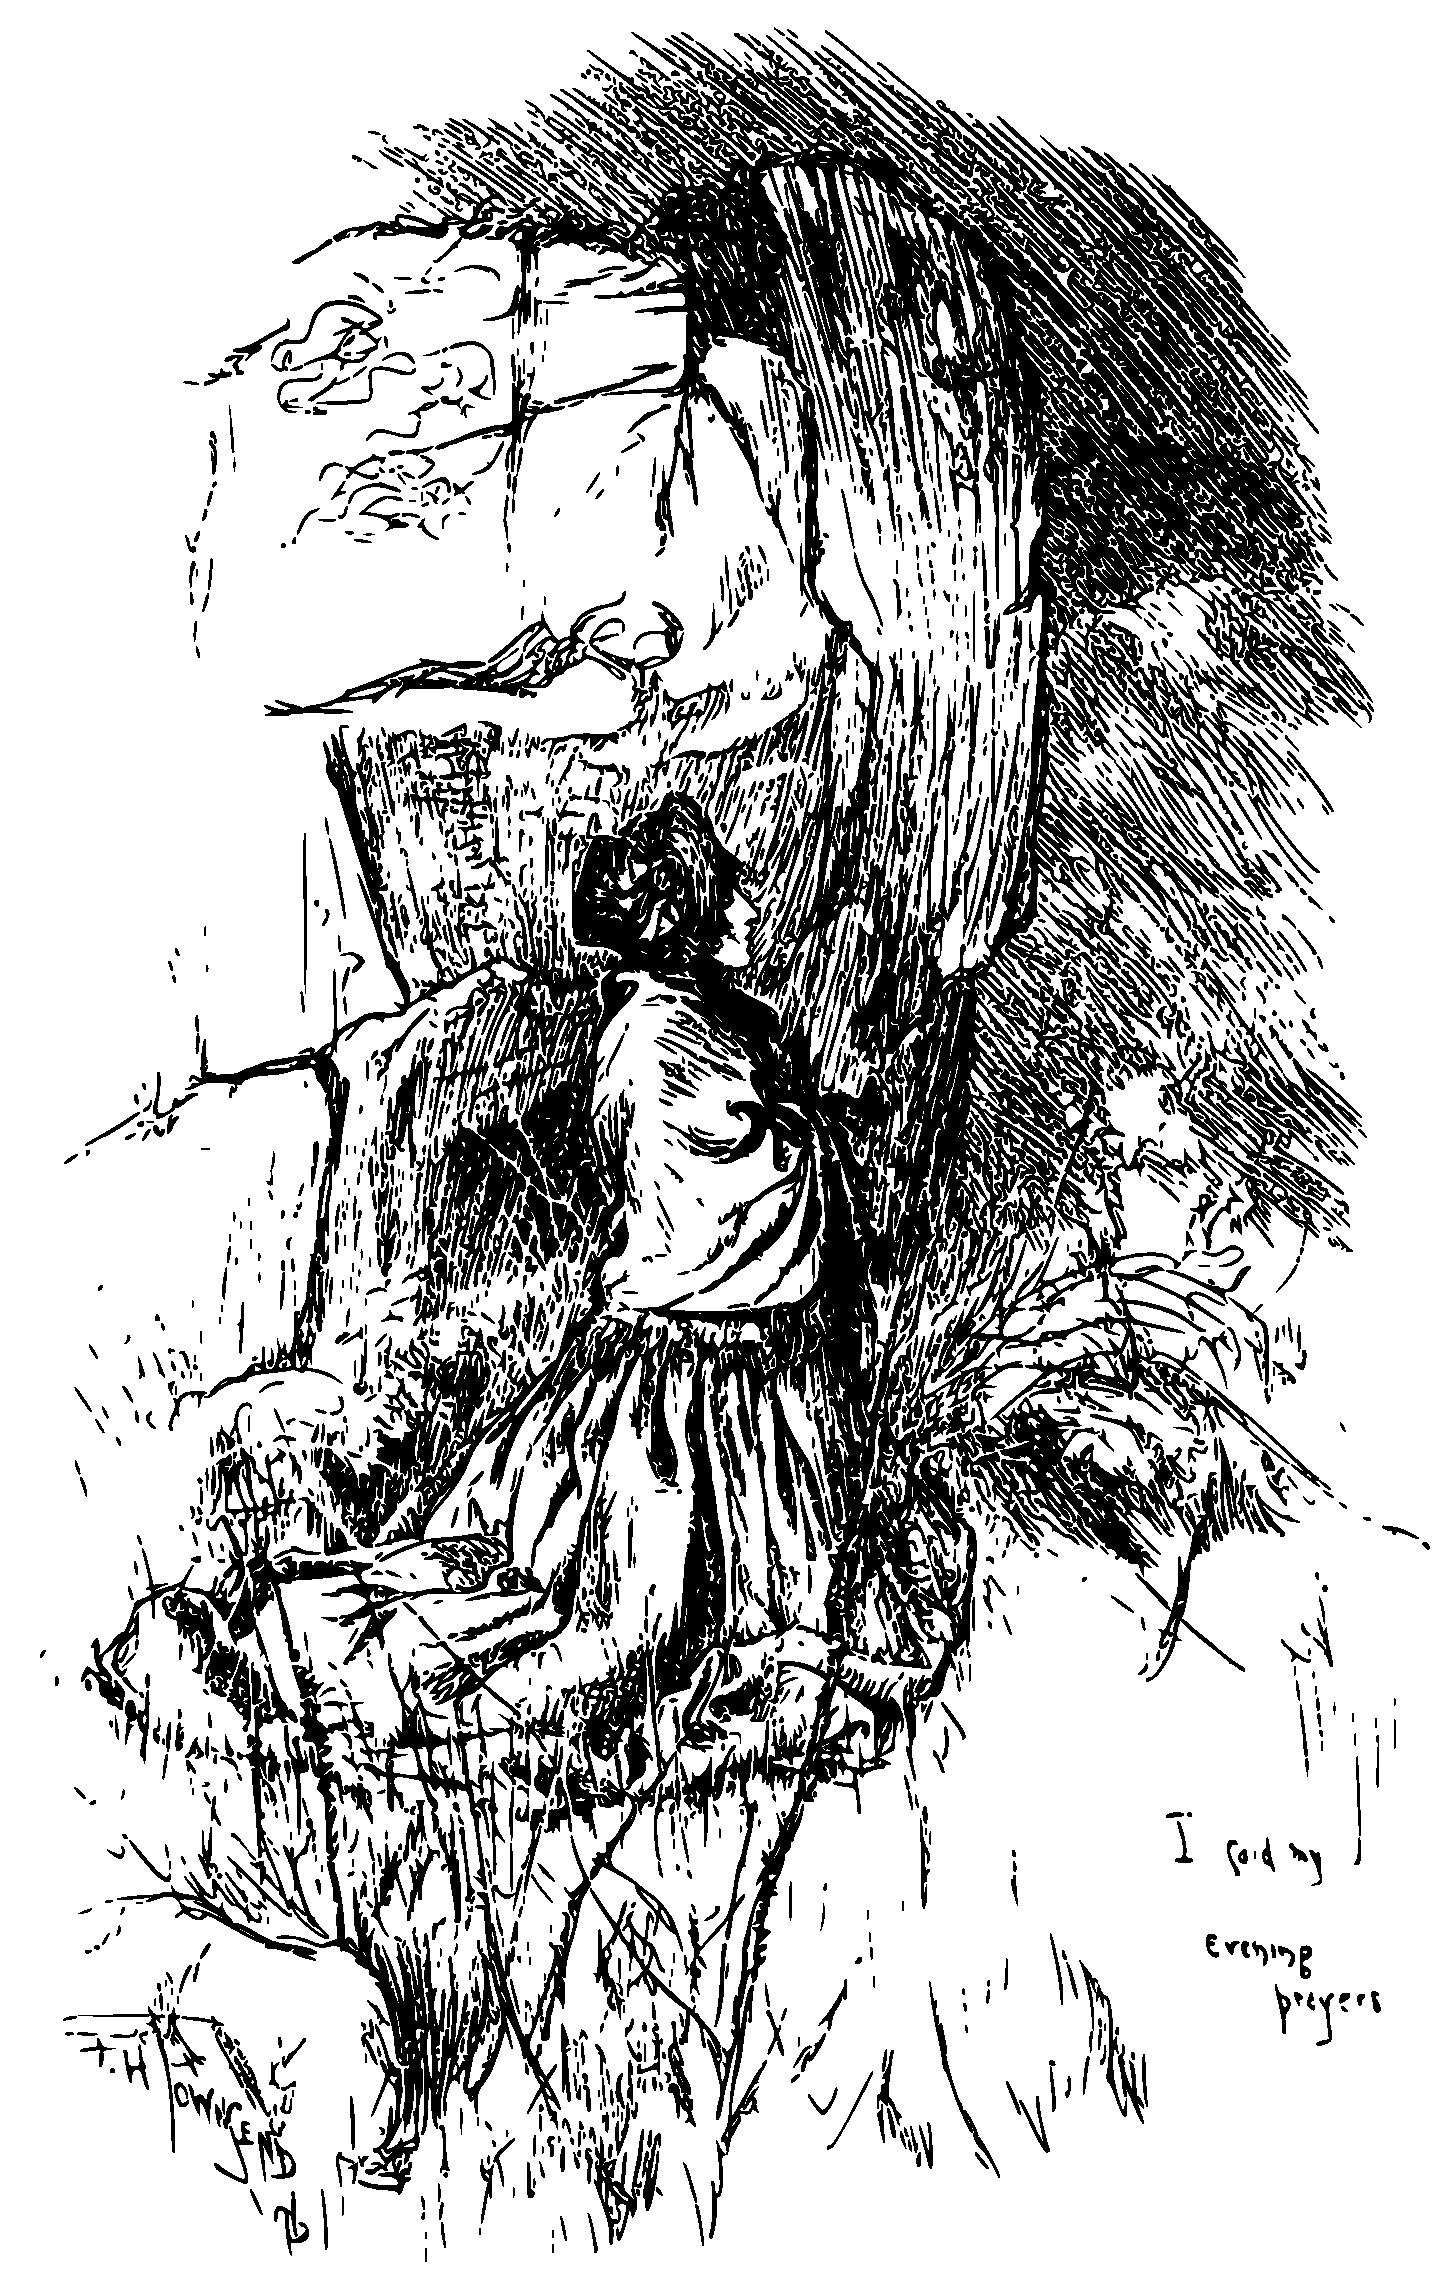
\includegraphics[width=\linewidth]{images/p311b.pdf}
	\end{sidecaption}
\end{figure}

Beside the crag the heath was very deep: when I lay down my feet were
buried in it; rising high on each side, it left only a narrow space for
the night-air to invade. I folded my shawl double, and spread it over
me for a coverlet; a low, mossy swell was my pillow. Thus lodged, I was
not, at least---at the commencement of the night, cold.

My rest might have been blissful enough, only a sad heart broke it. It
plained of its gaping wounds, its inward bleeding, its riven chords. It
trembled for \Mr{} Rochester and his doom; it bemoaned him with bitter
pity; it demanded him with ceaseless longing; and, impotent as a bird
with both wings broken, it still quivered its shattered pinions in vain
attempts to seek him.

Worn out with this torture of thought, I rose to my knees. Night was
come, and her planets were risen: a safe, still night: too serene for
the companionship of fear. We know that God is everywhere; but
certainly we feel His presence most when His works are on the grandest
scale spread before us; and it is in the unclouded night-sky, where His
worlds wheel their silent course, that we read clearest His infinitude,
His omnipotence, His omnipresence. I had risen to my knees to pray for
\Mr{} Rochester. Looking up, I, with tear-dimmed eyes, saw the mighty
Milky-way. Remembering what it was---what countless systems there swept
space like a soft trace of light---I felt the might and strength of
God. Sure was I of His efficiency to save what He had made: convinced I
grew that neither earth should perish, nor one of the souls it
treasured. I turned my prayer to thanksgiving: the Source of Life was
also the Saviour of spirits. \Mr{} Rochester was safe; he was God's, and
by God would he be guarded. I again nestled to the breast of the hill;
and ere long in sleep forgot sorrow.

But next day, Want came to me pale and bare. Long after the little
birds had left their nests; long after bees had come in the sweet prime
of day to gather the heath honey before the dew was dried---when the
long morning shadows were curtailed, and the sun filled earth and
sky---I got up, and I looked round me.

What a still, hot, perfect day! What a golden desert this spreading
moor! Everywhere sunshine. I wished I could live in it and on it. I
saw a lizard run over the crag; I saw a bee busy among the sweet
bilberries. I would fain at the moment have become bee or lizard, that
I might have found fitting nutriment, permanent shelter here. But I was
a human being, and had a human being's wants: I must not linger where
there was nothing to supply them. I rose; I looked back at the bed I
had left. Hopeless of the future, I wished but this---that my Maker had
that night thought good to require my soul of me while I slept; and that
this weary frame, absolved by death from further conflict with fate, had
now but to decay quietly, and mingle in peace with the soil of this
wilderness. Life, however, was yet in my possession, with all its
requirements, and pains, and responsibilities. The burden must be
carried; the want provided for; the suffering endured; the
responsibility fulfilled. I set out.

Whitcross regained, I followed a road which led from the sun, now
fervent and high. By no other circumstance had I will to decide my
choice. I walked a long time, and when I thought I had nearly done
enough, and might conscientiously yield to the fatigue that almost
overpowered me---might relax this forced action, and, sitting down on a
stone I saw near, submit resistlessly to the apathy that clogged heart
and limb---I heard a bell chime---a church bell.

I turned in the direction of the sound, and there, amongst the romantic
hills, whose changes and aspect I had ceased to note an hour ago, I saw
a hamlet and a spire. All the valley at my right hand was full of
pasture-fields, and cornfields, and wood; and a glittering stream ran
zig-zag through the varied shades of green, the mellowing grain, the
sombre woodland, the clear and sunny lea. Recalled by the rumbling of
wheels to the road before me, I saw a heavily-laden waggon labouring up
the hill, and not far beyond were two cows and their drover. Human life
and human labour were near. I must struggle on: strive to live and bend
to toil like the rest.

About two o'clock \PM{} I entered the village. At the bottom of its one
street there was a little shop with some cakes of bread in the window.
I coveted a cake of bread. With that refreshment I could perhaps regain
a degree of energy: without it, it would be difficult to proceed. The
wish to have some strength and some vigour returned to me as soon as I
was amongst my fellow-beings. I felt it would be degrading to faint
with hunger on the causeway of a hamlet. Had I nothing about me I could
offer in exchange for one of these rolls? I considered. I had a small
silk handkerchief tied round my throat; I had my gloves. I could hardly
tell how men and women in extremities of destitution proceeded. I did
not know whether either of these articles would be accepted: probably
they would not; but I must try.

I entered the shop: a woman was there. Seeing a respectably-dressed
person, a lady as she supposed, she came forward with civility. How
could she serve me? I was seized with shame: my tongue would not utter
the request I had prepared. I dared not offer her the half-worn gloves,
the creased handkerchief: besides, I felt it would be absurd. I only
begged permission to sit down a moment, as I was tired. Disappointed in
the expectation of a customer, she coolly acceded to my request. She
pointed to a seat; I sank into it. I felt sorely urged to weep; but
conscious how unseasonable such a manifestation would be, I restrained
it. Soon I asked her \enquote{if there were any dressmaker or
	plain-workwoman in the village?}

\enquote{Yes; two or three. Quite as many as there was employment for.}

I reflected. I was driven to the point now. I was brought face to face
with Necessity. I stood in the position of one without a resource,
without a friend, without a coin. I must do something. What? I must
apply somewhere. Where?

\enquote{Did she know of any place in the neighbourhood where a servant
	was wanted?}

\enquote{Nay; she couldn't say.}

\enquote{What was the chief trade in this place? What did most of the
	people do?}

\enquote{Some were farm labourers; a good deal worked at \Mr{} Oliver's
	needle-factory, and at the foundry.}

\enquote{Did \Mr{} Oliver employ women?}

\enquote{Nay; it was men's work.}

\enquote{And what do the women do?}

\enquote{I knawn't,} was the answer. \enquote{Some does one thing, and
	some another. Poor folk mun get on as they can.}

She seemed to be tired of my questions: and, indeed, what claim had I to
importune her? A neighbour or two came in; my chair was evidently
wanted. I took leave.

I passed up the street, looking as I went at all the houses to the right
hand and to the left; but I could discover no pretext, nor see an
inducement to enter any. I rambled round the hamlet, going sometimes to
a little distance and returning again, for an hour or more. Much
exhausted, and suffering greatly now for want of food, I turned aside
into a lane and sat down under the hedge. Ere many minutes had elapsed,
I was again on my feet, however, and again searching something---a
resource, or at least an informant. A pretty little house stood at the
top of the lane, with a garden before it, exquisitely neat and
brilliantly blooming. I stopped at it. What business had I to approach
the white door or touch the glittering knocker? In what way could it
possibly be the interest of the inhabitants of that dwelling to serve
me? Yet I drew near and knocked. A mild-looking, cleanly-attired young
woman opened the door. In such a voice as might be expected from a
hopeless heart and fainting frame---a voice wretchedly low and
faltering---I asked if a servant was wanted here?

\enquote{No,} said she; \enquote{we do not keep a servant.}

\enquote{Can you tell me where I could get employment of any kind?} I
continued. \enquote{I am a stranger, without acquaintance in this
	place. I want some work: no matter what.}

But it was not her business to think for me, or to seek a place for me:
besides, in her eyes, how doubtful must have appeared my character,
position, tale. She shook her head, she \enquote{was sorry she could
	give me no information,} and the white door closed, quite gently and
civilly: but it shut me out. If she had held it open a little longer, I
believe I should have begged a piece of bread; for I was now brought
low.

I could not bear to return to the sordid village, where, besides, no
prospect of aid was visible. I should have longed rather to deviate to
a wood I saw not far off, which appeared in its thick shade to offer
inviting shelter; but I was so sick, so weak, so gnawed with nature's
cravings, instinct kept me roaming round abodes where there was a chance
of food. Solitude would be no solitude---rest no rest---while the
vulture, hunger, thus sank beak and talons in my side.

I drew near houses; I left them, and came back again, and again I
wandered away: always repelled by the consciousness of having no claim
to ask---no right to expect interest in my isolated lot. Meantime, the
afternoon advanced, while I thus wandered about like a lost and starving
dog. In crossing a field, I saw the church spire before me: I hastened
towards it. Near the churchyard, and in the middle of a garden, stood a
well-built though small house, which I had no doubt was the parsonage.
I remembered that strangers who arrive at a place where they have no
friends, and who want employment, sometimes apply to the clergyman for
introduction and aid. It is the clergyman's function to help---at least
with advice---those who wished to help themselves. I seemed to have
something like a right to seek counsel here. Renewing then my courage,
and gathering my feeble remains of strength, I pushed on. I reached the
house, and knocked at the kitchen-door. An old woman opened: I asked
was this the parsonage?

\enquote{Yes.}

\enquote{Was the clergyman in?}

\enquote{No.}

\enquote{Would he be in soon?}

\enquote{No, he was gone from home.}

\enquote{To a distance?}

\enquote{Not so far---happen three mile. He had been called away by the
	sudden death of his father: he was at Marsh End now, and would very
	likely stay there a fortnight longer.}

\enquote{Was there any lady of the house?}

\enquote{Nay, there was naught but her, and she was housekeeper;} and of
her, reader, I could not bear to ask the relief for want of which I was
sinking; I could not yet beg; and again I crawled away.

Once more I took off my handkerchief---once more I thought of the cakes
of bread in the little shop. Oh, for but a crust! for but one mouthful
to allay the pang of famine! Instinctively I turned my face again to
the village; I found the shop again, and I went in; and though others
were there besides the woman I ventured the request---\enquote{Would she
	give me a roll for this handkerchief?}

She looked at me with evident suspicion: \enquote{Nay, she never sold
	stuff i' that way.}

Almost desperate, I asked for half a cake; she again refused.
\enquote{How could she tell where I had got the handkerchief?} she said.

\enquote{Would she take my gloves?}

\enquote{No! what could she do with them?}

Reader, it is not pleasant to dwell on these details. Some say there is
enjoyment in looking back to painful experience past; but at this day I
can scarcely bear to review the times to which I allude: the moral
degradation, blent with the physical suffering, form too distressing a
recollection ever to be willingly dwelt on. I blamed none of those who
repulsed me. I felt it was what was to be expected, and what could not
be helped: an ordinary beggar is frequently an object of suspicion; a
well-dressed beggar inevitably so. To be sure, what I begged was
employment; but whose business was it to provide me with employment?
Not, certainly, that of persons who saw me then for the first time, and
who knew nothing about my character. And as to the woman who would not
take my handkerchief in exchange for her bread, why, she was right, if
the offer appeared to her sinister or the exchange unprofitable. Let me
condense now. I am sick of the subject.

A little before dark I passed a farm-house, at the open door of which
the farmer was sitting, eating his supper of bread and cheese. I
stopped and said---

\enquote{Will you give me a piece of bread? for I am very hungry.} He
cast on me a glance of surprise; but without answering, he cut a thick
slice from his loaf, and gave it to me. I imagine he did not think I
was a beggar, but only an eccentric sort of lady, who had taken a fancy
to his brown loaf. As soon as I was out of sight of his house, I sat
down and ate it.

I could not hope to get a lodging under a roof, and sought it in the
wood I have before alluded to. But my night was wretched, my rest
broken: the ground was damp, the air cold: besides, intruders passed
near me more than once, and I had again and again to change my quarters;
no sense of safety or tranquillity befriended me. Towards morning it
rained; the whole of the following day was wet. Do not ask me, reader,
to give a minute account of that day; as before, I sought work; as
before, I was repulsed; as before, I starved; but once did food pass my
lips. At the door of a cottage I saw a little girl about to throw a
mess of cold porridge into a pig trough. \enquote{Will you give me
	that?} I asked.

\begin{figure}
	\begin{sidecaption}{\enquote{Will you give me that?}\linebreak I asked.}[p316b]
		\centering
		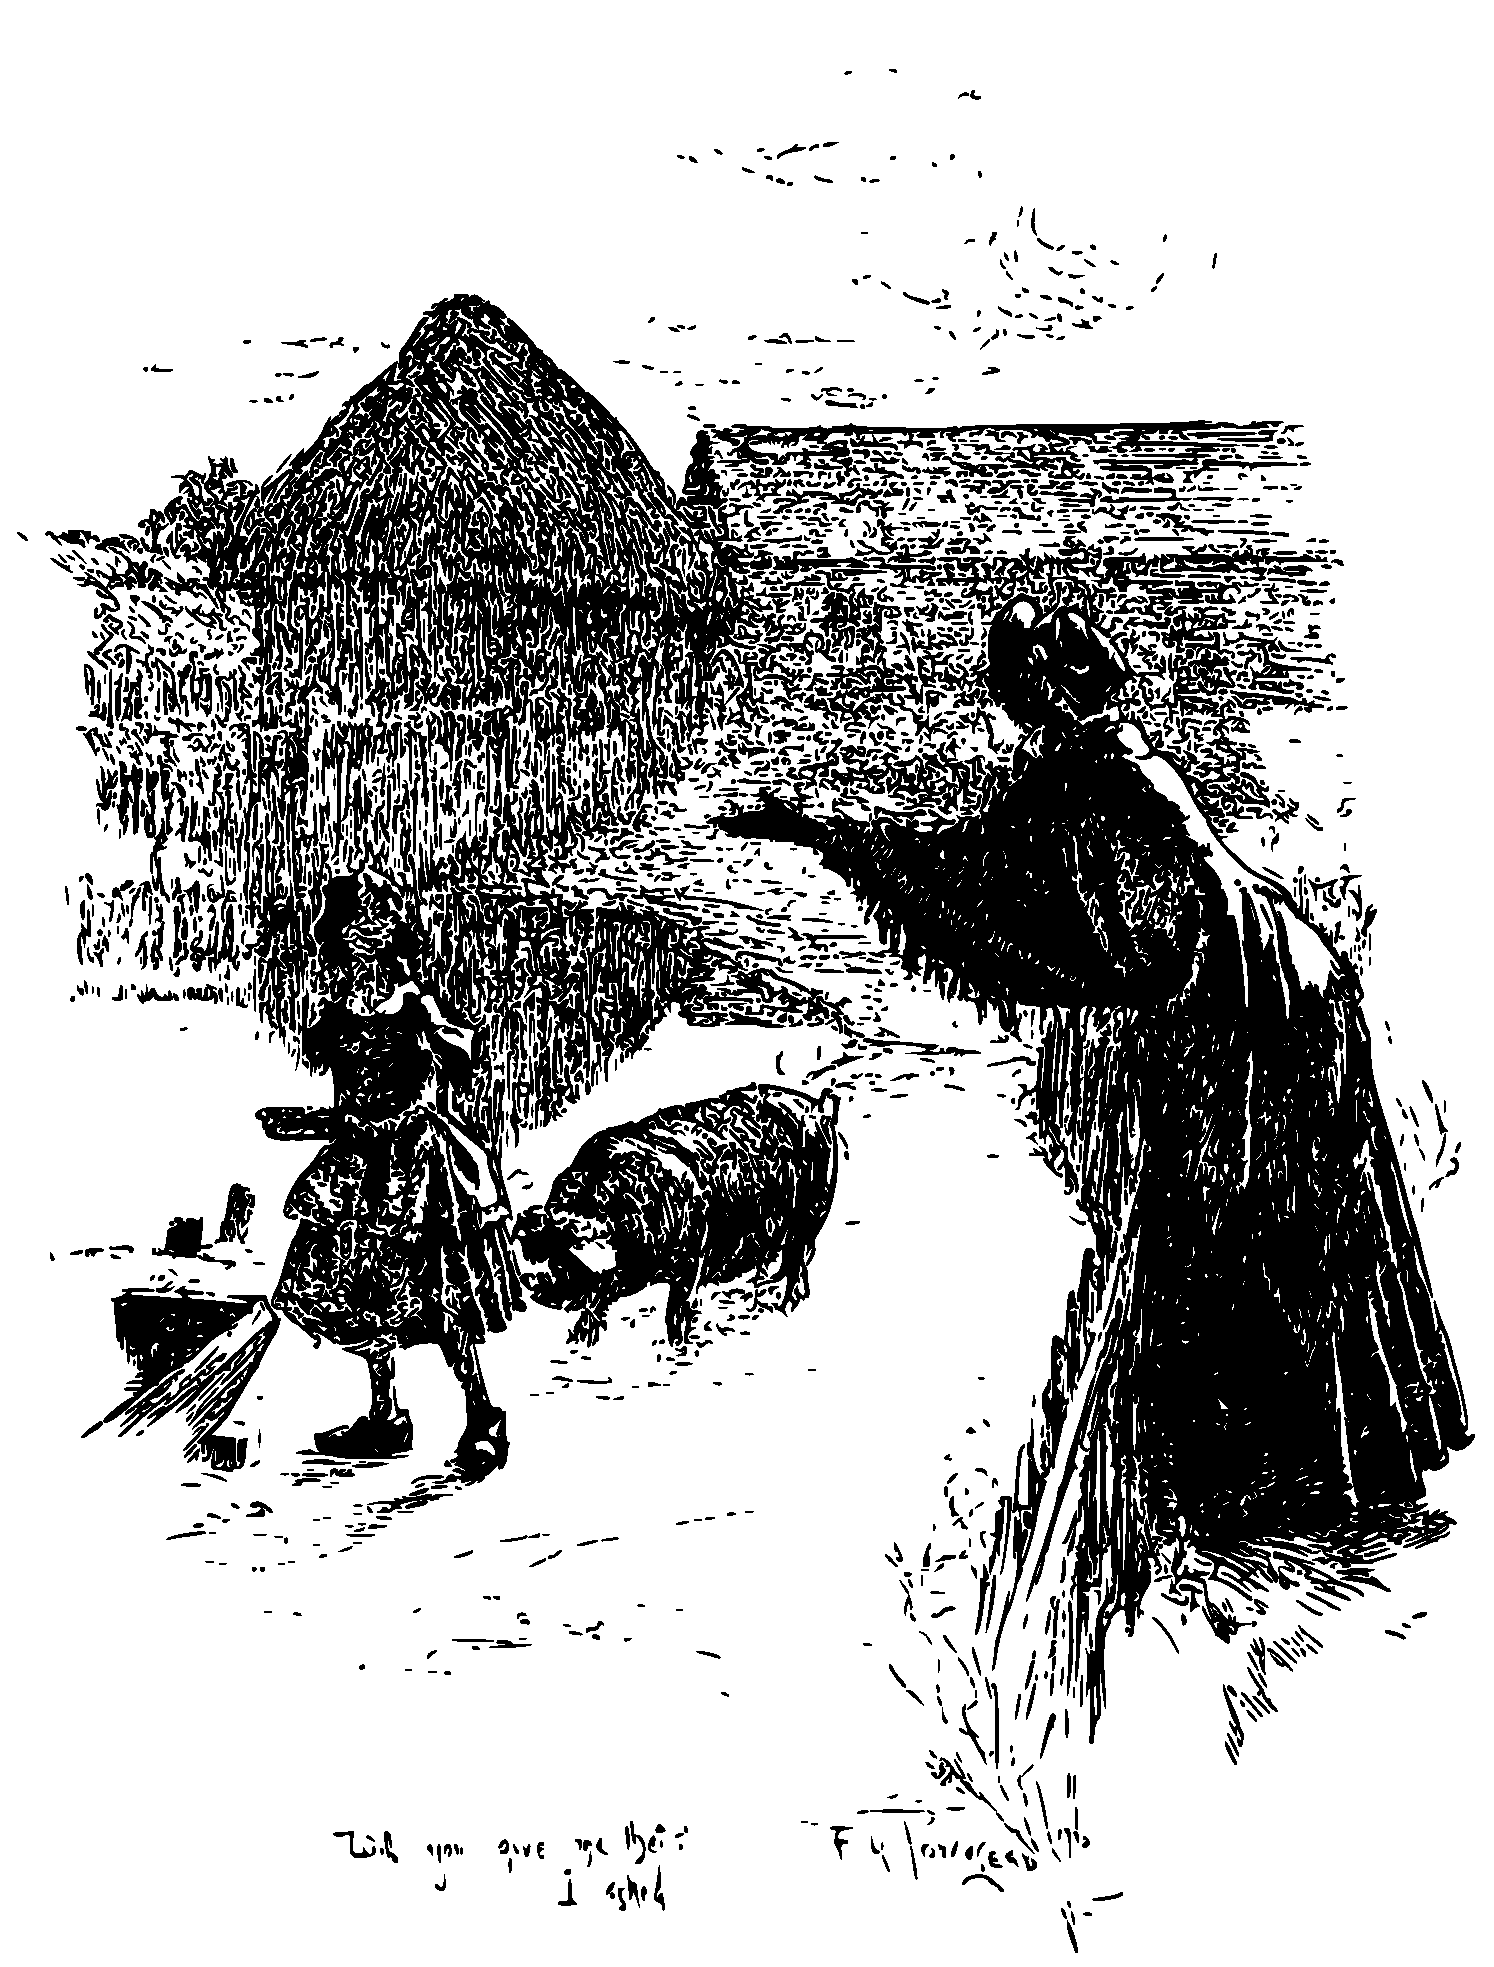
\includegraphics[width=\linewidth]{images/p316b.pdf}
	\end{sidecaption}
\end{figure}

She stared at me. \enquote{Mother!} she exclaimed, \enquote{there is a
	woman wants me to give her these porridge.}

\enquote{Well lass,} replied a voice within, \enquote{give it her if
	she's a beggar. T' pig doesn't want it.}

The girl emptied the stiffened mould into my hand, and I devoured it
ravenously.

As the wet twilight deepened, I stopped in a solitary bridle-path, which
I had been pursuing an hour or more.

\enquote{My strength is quite failing me,} I said in a soliloquy.
\enquote{I feel I cannot go much farther. Shall I be an outcast again
	this night? While the rain descends so, must I lay my head on the cold,
	drenched ground? I fear I cannot do otherwise: for who will receive
	me? But it will be very dreadful, with this feeling of hunger,
	faintness, chill, and this sense of desolation---this total prostration
	of hope. In all likelihood, though, I should die before morning. And
	why cannot I reconcile myself to the prospect of death? Why do I
	struggle to retain a valueless life? Because I know, or believe, \Mr{}
	Rochester is living: and then, to die of want and cold is a fate to
	which nature cannot submit passively. Oh, Providence! sustain me a
	little longer! Aid!---direct me!}

My glazed eye wandered over the dim and misty landscape. I saw I had
strayed far from the village: it was quite out of sight. The very
cultivation surrounding it had disappeared. I had, by cross-ways and
by-paths, once more drawn near the tract of moorland; and now, only a
few fields, almost as wild and unproductive as the heath from which they
were scarcely reclaimed, lay between me and the dusky hill.

\enquote{Well, I would rather die yonder than in a street or on a
	frequented road,} I reflected. \enquote{And far better that crows and
	ravens---if any ravens there be in these regions---should pick my flesh
	from my bones, than that they should be prisoned in a workhouse coffin
	and moulder in a pauper's grave.}

To the hill, then, I turned. I reached it. It remained now only to
find a hollow where I could lie down, and feel at least hidden, if not
secure. But all the surface of the waste looked level. It showed no
variation but of tint: green, where rush and moss overgrew the marshes;
black, where the dry soil bore only heath. Dark as it was getting, I
could still see these changes, though but as mere alternations of light
and shade; for colour had faded with the daylight.

My eye still roved over the sullen swell and along the moor-edge,
vanishing amidst the wildest scenery, when at one dim point, far in
among the marshes and the ridges, a light sprang up. \enquote{That is an
	\emph{ignis fatuus},} was my first thought; and I expected it would
soon vanish. It burnt on, however, quite steadily, neither receding nor
advancing. \enquote{Is it, then, a bonfire just kindled?} I
questioned. I watched to see whether it would spread: but no; as it did
not diminish, so it did not enlarge. \enquote{It may be a candle in a
	house,} I then conjectured; \enquote{but if so, I can never reach it.
	It is much too far away: and were it within a yard of me, what would it
	avail? I should but knock at the door to have it shut in my face.}

And I sank down where I stood, and hid my face against the ground. I
lay still a while: the night-wind swept over the hill and over me, and
died moaning in the distance; the rain fell fast, wetting me afresh to
the skin. Could I but have stiffened to the still frost---the friendly
numbness of death---it might have pelted on; I should not have felt it;
but my yet living flesh shuddered at its chilling influence. I rose ere
long.

The light was yet there, shining dim but constant through the rain. I
tried to walk again: I dragged my exhausted limbs slowly towards it. It
led me aslant over the hill, through a wide bog, which would have been
impassable in winter, and was splashy and shaking even now, in the
height of summer. Here I fell twice; but as often I rose and rallied my
faculties. This light was my forlorn hope: I must gain it.

Having crossed the marsh, I saw a trace of white over the moor. I
approached it; it was a road or a track: it led straight up to the
light, which now beamed from a sort of knoll, amidst a clump of
trees---firs, apparently, from what I could distinguish of the character
of their forms and foliage through the gloom. My star vanished as I
drew near: some obstacle had intervened between me and it. I put out my
hand to feel the dark mass before me: I discriminated the rough stones
of a low wall---above it, something like palisades, and within, a high
and prickly hedge. I groped on. Again a whitish object gleamed before
me: it was a gate---a wicket; it moved on its hinges as I touched it.
On each side stood a sable bush-holly or yew.

Entering the gate and passing the shrubs, the silhouette of a house rose
to view, black, low, and rather long; but the guiding light shone
nowhere. All was obscurity. Were the inmates retired to rest? I
feared it must be so. In seeking the door, I turned an angle: there
shot out the friendly gleam again, from the lozenged panes of a very
small latticed window, within a foot of the ground, made still smaller
by the growth of ivy or some other creeping plant, whose leaves
clustered thick over the portion of the house wall in which it was set.
The aperture was so screened and narrow, that curtain or shutter had
been deemed unnecessary; and when I stooped down and put aside the spray
of foliage shooting over it, I could see all within. I could see
clearly a room with a sanded floor, clean scoured; a dresser of walnut,
with pewter plates ranged in rows, reflecting the redness and radiance
of a glowing peat-fire. I could see a clock, a white deal table, some
chairs. The candle, whose ray had been my beacon, burnt on the table;
and by its light an elderly woman, somewhat rough-looking, but
scrupulously clean, like all about her, was knitting a stocking.

I noticed these objects cursorily only---in them there was nothing
extraordinary. A group of more interest appeared near the hearth,
sitting still amidst the rosy peace and warmth suffusing it. Two young,
graceful women---ladies in every point---sat, one in a low
rocking-chair, the other on a lower stool; both wore deep mourning of
crape and bombazeen, which sombre garb singularly set off very fair
necks and faces: a large old pointer dog rested its massive head on the
knee of one girl---in the lap of the other was cushioned a black cat.

A strange place was this humble kitchen for such occupants! Who were
they? They could not be the daughters of the elderly person at the
table; for she looked like a rustic, and they were all delicacy and
cultivation. I had nowhere seen such faces as theirs: and yet, as I
gazed on them, I seemed intimate with every lineament. I cannot call
them handsome---they were too pale and grave for the word: as they each
bent over a book, they looked thoughtful almost to severity. A stand
between them supported a second candle and two great volumes, to which
they frequently referred, comparing them, seemingly, with the smaller
books they held in their hands, like people consulting a dictionary to
aid them in the task of translation. This scene was as silent as if all
the figures had been shadows and the firelit apartment a picture: so
hushed was it, I could hear the cinders fall from the grate, the clock
tick in its obscure corner; and I even fancied I could distinguish the
click-click of the woman's knitting-needles. When, therefore, a voice
broke the strange stillness at last, it was audible enough to me.

\enquote{Listen, Diana,} said one of the absorbed students;
\enquote{Franz and old Daniel are together in the night-time, and Franz
	is telling a dream from which he has awakened in terror---listen!} And
in a low voice she read something, of which not one word was
intelligible to me; for it was in an unknown tongue---neither French nor
Latin. Whether it were Greek or German I could not tell.

\enquote{That is strong,} she said, when she had finished: \enquote{I
	relish it.} The other girl, who had lifted her head to listen to her
sister, repeated, while she gazed at the fire, a line of what had been
read. At a later day, I knew the language and the book; therefore, I
will here quote the line: though, when I first heard it, it was only
like a stroke on sounding brass to me---conveying no meaning:---

\enquote{\foreignquote{german}{Da trat hervor Einer, anzusehen wie die Sternen
		Nacht.}\footnote{\enquote{Then one stepped forth, who appeared like the stars of the night.}}
	Good! good!} she exclaimed, while her dark and deep eye
sparkled. \enquote{There you have a dim and mighty archangel fitly set
	before you! The line is worth a hundred pages of fustian.
	\foreignquote{german}{Ich wäge die Gedanken in der Schale meines Zornes und die
		Werke mit dem Gewichte meines Grimms.}\footnote{
		\enquote{I weigh thoughts in the scale of my anger and works against the weight of my wrath.}} I like it!}

Both were again silent.

\enquote{Is there ony country where they talk i' that way?} asked the
old woman, looking up from her knitting.

\enquote{Yes, Hannah---a far larger country than England, where they
	talk in no other way.}

\enquote{Well, for sure case, I knawn't how they can understand t' one
	t'other: and if either o' ye went there, ye could tell what they said, I
	guess?}

\enquote{We could probably tell something of what they said, but not
	all---for we are not as clever as you think us, Hannah. We don't speak
	German, and we cannot read it without a dictionary to help us.}

\enquote{And what good does it do you?}

\enquote{We mean to teach it some time---or at least the elements, as
	they say; and then we shall get more money than we do now.}

\enquote{Varry like: but give ower studying; ye've done enough for
	to-night.}

\enquote{I think we have: at least I'm tired. Mary, are you?}

\enquote{Mortally: after all, it's tough work fagging away at a language
	with no master but a lexicon.}

\enquote{It is, especially such a language as this crabbed but glorious
	Deutsch. I wonder when \St{} John will come home.}

\enquote{Surely he will not be long now: it is just ten (looking at a
	little gold watch she drew from her girdle). It rains fast, Hannah:
	will you have the goodness to look at the fire in the parlour?}

The woman rose: she opened a door, through which I dimly saw a passage:
soon I heard her stir a fire in an inner room; she presently came back.

\enquote{Ah, childer!} said she, \enquote{it fair troubles me to go into
	yond' room now: it looks so lonesome wi' the chair empty and set back in
	a corner.}

She wiped her eyes with her apron: the two girls, grave before, looked
sad now.

\enquote{But he is in a better place,} continued Hannah: \enquote{we
	shouldn't wish him here again. And then, nobody need to have a quieter
	death nor he had.}

\enquote{You say he never mentioned us?} inquired one of the ladies.

\enquote{He hadn't time, bairn: he was gone in a minute, was your
	father. He had been a bit ailing like the day before, but naught to
	signify; and when \Mr{} \St{} John asked if he would like either o' ye to be
	sent for, he fair laughed at him. He began again with a bit of a
	heaviness in his head the next day---that is, a fortnight sin'---and he
	went to sleep and niver wakened: he wor a'most stark when your brother
	went into t' chamber and fand him. Ah, childer! that's t' last o' t'
	old stock---for ye and \Mr{} \St{} John is like of different soart to them
	\enquote{at's gone; for all your mother wor mich i} your way, and
	a'most as book-learned. She wor the pictur' o' ye, Mary: Diana is more
	like your father.}

I thought them so similar I could not tell where the old servant (for
such I now concluded her to be) saw the difference. Both were fair
complexioned and slenderly made; both possessed faces full of
distinction and intelligence. One, to be sure, had hair a shade darker
than the other, and there was a difference in their style of wearing it;
Mary's pale brown locks were parted and braided smooth: Diana's duskier
tresses covered her neck with thick curls. The clock struck ten.

\enquote{Ye'll want your supper, I am sure,} observed Hannah;
\enquote{and so will \Mr{} \St{} John when he comes in.}

And she proceeded to prepare the meal. The ladies rose; they seemed
about to withdraw to the parlour. Till this moment, I had been so
intent on watching them, their appearance and conversation had excited
in me so keen an interest, I had half-forgotten my own wretched
position: now it recurred to me. More desolate, more desperate than
ever, it seemed from contrast. And how impossible did it appear to
touch the inmates of this house with concern on my behalf; to make them
believe in the truth of my wants and woes---to induce them to vouchsafe
a rest for my wanderings! As I groped out the door, and knocked at it
hesitatingly, I felt that last idea to be a mere chimera. Hannah
opened.

\enquote{What do you want?} she inquired, in a voice of surprise, as she
surveyed me by the light of the candle she held.

\enquote{May I speak to your mistresses?} I said.

\enquote{You had better tell me what you have to say to them. Where do
	you come from?}

\enquote{I am a stranger.}

\enquote{What is your business here at this hour?}

\enquote{I want a night's shelter in an out-house or anywhere, and a
	morsel of bread to eat.}

Distrust, the very feeling I dreaded, appeared in Hannah's face.
\enquote{I'll give you a piece of bread,} she said, after a pause;
\enquote{but we can't take in a vagrant to lodge. It isn't likely.}

\enquote{Do let me speak to your mistresses.}

\enquote{No, not I\@. What can they do for you? You should not be roving
	about now; it looks very ill.}

\enquote{But where shall I go if you drive me away? What shall I do?}

\enquote{Oh, I'll warrant you know where to go and what to do. Mind you
	don't do wrong, that's all. Here is a penny; now go---}

\enquote{A penny cannot feed me, and I have no strength to go farther.
	Don't shut the door:---oh, don't, for God's sake!}

\enquote{I must; the rain is driving in---}

\enquote{Tell the young ladies. Let me see them---}

\enquote{Indeed, I will not. You are not what you ought to be, or you
	wouldn't make such a noise. Move off.}

\enquote{But I must die if I am turned away.}

\enquote{Not you. I'm fear'd you have some ill plans agate, that bring
	you about folk's houses at this time o' night. If you've any
	followers---housebreakers or such like---anywhere near, you may tell
	them we are not by ourselves in the house; we have a gentleman, and
	dogs, and guns.} Here the honest but inflexible servant clapped the
door to and bolted it within.

This was the climax. A pang of exquisite suffering---a throe of true
despair---rent and heaved my heart. Worn out, indeed, I was; not
another step could I stir. I sank on the wet doorstep: I groaned---I
wrung my hands---I wept in utter anguish. Oh, this spectre of death!
Oh, this last hour, approaching in such horror! Alas, this
isolation---this banishment from my kind! Not only the anchor of hope,
but the footing of fortitude was gone---at least for a moment; but the
last I soon endeavoured to regain.

\enquote{I can but die,} I said, \enquote{and I believe in God. Let me
	try to wait His will in silence.}

These words I not only thought, but uttered; and thrusting back all my
misery into my heart, I made an effort to compel it to remain
there---dumb and still.

\enquote{All men must die,} said a voice quite close at hand;
\enquote{but all are not condemned to meet a lingering and premature
	doom, such as yours would be if you perished here of want.}

\enquote{Who or what speaks?} I asked, terrified at the unexpected
sound, and incapable now of deriving from any occurrence a hope of aid.
A form was near---what form, the pitch-dark night and my enfeebled
vision prevented me from distinguishing. With a loud long knock, the
new-comer appealed to the door.

\enquote{Is it you, \Mr{} \St{} John?} cried Hannah.

\enquote{Yes---yes; open quickly.}

\enquote{Well, how wet and cold you must be, such a wild night as it
	is! Come in---your sisters are quite uneasy about you, and I believe
	there are bad folks about. There has been a beggar-woman---I declare
	she is not gone yet!---laid down there. Get up! for shame! Move off, I
	say!}

\enquote{Hush, Hannah! I have a word to say to the woman. You have
	done your duty in excluding, now let me do mine in admitting her. I was
	near, and listened to both you and her. I think this is a peculiar
	case---I must at least examine into it. Young woman, rise, and pass
	before me into the house.}

\begin{figure}
	\begin{sidecaption}{\enquote{Hush, Hannah!\linebreak I have a word\linebreak to say to the woman.}}[p323b]
		\centering
		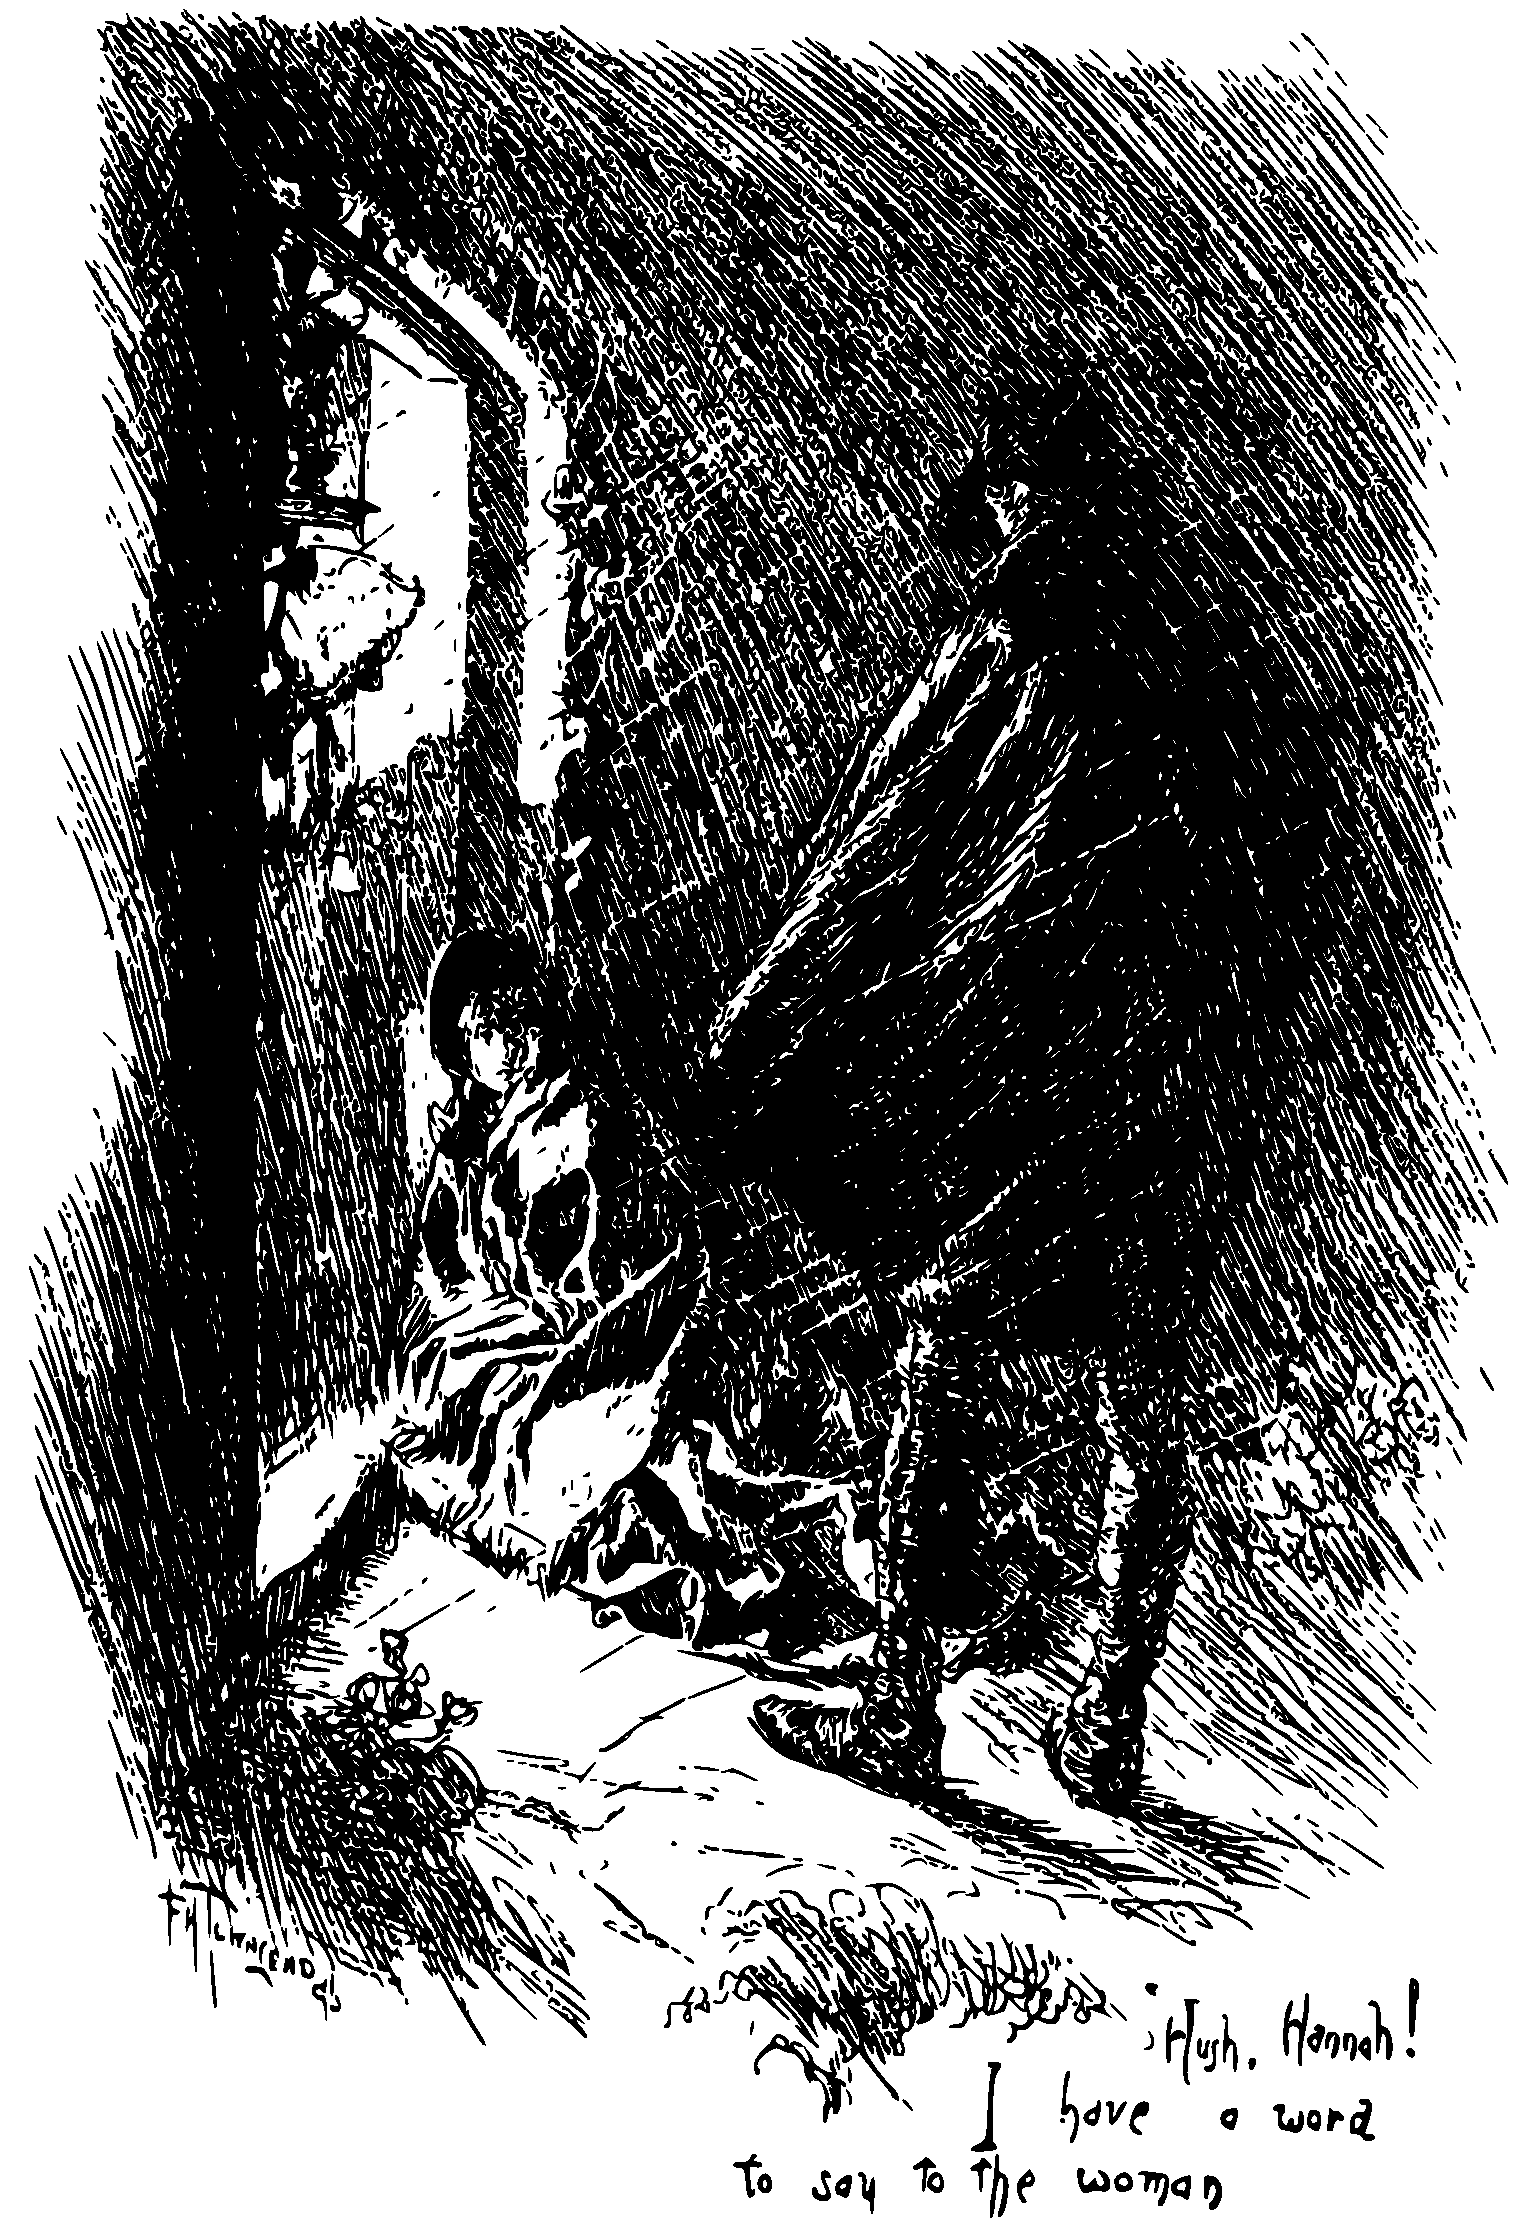
\includegraphics[width=\linewidth]{images/p323b.pdf}
	\end{sidecaption}
\end{figure}

With difficulty I obeyed him. Presently I stood within that clean,
bright kitchen---on the very hearth---trembling, sickening; conscious of
an aspect in the last degree ghastly, wild, and weather-beaten. The two
ladies, their brother, \Mr{} \St{} John, the old servant, were all gazing at
me.

\enquote{\St{} John, who is it?} I heard one ask.

\enquote{I cannot tell: I found her at the door,} was the reply.

\enquote{She does look white,} said Hannah.

\enquote{As white as clay or death,} was responded. \enquote{She will
	fall: let her sit.}

And indeed my head swam: I dropped, but a chair received me. I still
possessed my senses, though just now I could not speak.

\enquote{Perhaps a little water would restore her. Hannah, fetch some.
	But she is worn to nothing. How very thin, and how very bloodless!}

\enquote{A mere spectre!}

\enquote{Is she ill, or only famished?}

\enquote{Famished, I think. Hannah, is that milk? Give it me, and a
	piece of bread.}

Diana (I knew her by the long curls which I saw drooping between me and
the fire as she bent over me) broke some bread, dipped it in milk, and
put it to my lips. Her face was near mine: I saw there was pity in it,
and I felt sympathy in her hurried breathing. In her simple words, too,
the same balm-like emotion spoke: \enquote{Try to eat.}

\enquote{Yes---try,} repeated Mary gently; and Mary's hand removed my
sodden bonnet and lifted my head. I tasted what they offered me: feebly
at first, eagerly soon.

\enquote{Not too much at first---restrain her,} said the brother;
\enquote{she has had enough.} And he withdrew the cup of milk and the
plate of bread.

\enquote{A little more, \St{} John---look at the avidity in her eyes.}

\enquote{No more at present, sister. Try if she can speak now---ask her
	her name.}

I felt I could speak, and I answered---\enquote{My name is Jane
	Elliott.} Anxious as ever to avoid discovery, I had before resolved to
assume an \emph{alias}.

\enquote{And where do you live? Where are your friends?}

I was silent.

\enquote{Can we send for any one you know?}

I shook my head.

\enquote{What account can you give of yourself?}

Somehow, now that I had once crossed the threshold of this house, and
once was brought face to face with its owners, I felt no longer outcast,
vagrant, and disowned by the wide world. I dared to put off the
mendicant---to resume my natural manner and character. I began once
more to know myself; and when \Mr{} \St{} John demanded an account---which
at present I was far too weak to render---I said after a brief pause---

\enquote{Sir, I can give you no details to-night.}

\enquote{But what, then,} said he, \enquote{do you expect me to do for
	you?}

\enquote{Nothing,} I replied. My strength sufficed for but short
answers. Diana took the word---

\enquote{Do you mean,} she asked, \enquote{that we have now given you
	what aid you require? and that we may dismiss you to the moor and the
	rainy night?}

I looked at her. She had, I thought, a remarkable countenance, instinct
both with power and goodness. I took sudden courage. Answering her
compassionate gaze with a smile, I said---\enquote{I will trust you. If
	I were a masterless and stray dog, I know that you would not turn me
	from your hearth to-night: as it is, I really have no fear. Do with me
	and for me as you like; but excuse me from much discourse---my breath is
	short---I feel a spasm when I speak.} All three surveyed me, and all
three were silent.

\enquote{Hannah,} said \Mr{} \St{} John, at last, \enquote{let her sit there
	at present, and ask her no questions; in ten minutes more, give her the
	remainder of that milk and bread. Mary and Diana, let us go into the
	parlour and talk the matter over.}

They withdrew. Very soon one of the ladies returned---I could not tell
which. A kind of pleasant stupor was stealing over me as I sat by the
genial fire. In an undertone she gave some directions to Hannah. Ere
long, with the servant's aid, I contrived to mount a staircase; my
dripping clothes were removed; soon a warm, dry bed received me. I
thanked God---experienced amidst unutterable exhaustion a glow of
grateful joy---and slept.
